%%%%%%%%%%%%%%%%%%%%%%%%%%%%%%%%%%%%%%%%%
% Tufte-Style Book (Minimal Template)
% LaTeX Template
% Version 1.0 (5/1/13)
%
% This template has been downloaded from:
% http://www.LaTeXTemplates.com
%
% License:
% CC BY-NC-SA 3.0 (http://creativecommons.org/licenses/by-nc-sa/3.0/)
%
% IMPORTANT NOTE:
% In addition to running BibTeX to compile the reference list from the .bib
% file, you will need to run MakeIndex to compile the index at the end of the
% document.
%
%%%%%%%%%%%%%%%%%%%%%%%%%%%%%%%%%%%%%%%%%

%----------------------------------------------------------------------------------------
%	PACKAGES AND OTHER DOCUMENT CONFIGURATIONS
%----------------------------------------------------------------------------------------

\documentclass{tufte-book} % Use the tufte-book class which in turn uses the tufte-common class

\hypersetup{colorlinks} % Comment this line if you don't wish to have colored links

\usepackage{microtype} % Improves character and word spacing

\usepackage{lipsum} % Inserts dummy text

\usepackage{booktabs} % Better horizontal rules in tables

\usepackage{graphicx} % Needed to insert images into the document
\graphicspath{{graphics/}} % Sets the default location of pictures
\setkeys{Gin}{width=\linewidth,totalheight=\textheight,keepaspectratio} % Improves figure scaling

\usepackage{fancyvrb} % Allows customization of verbatim environments
\fvset{fontsize=\normalsize} % The font size of all verbatim text can be changed here

\newcommand{\hangp}[1]{\makebox[0pt][r]{(}#1\makebox[0pt][l]{)}} % New command to create parentheses around text in tables which take up no horizontal space - this improves column spacing
\newcommand{\hangstar}{\makebox[0pt][l]{*}} % New command to create asterisks in tables which take up no horizontal space - this improves column spacing

\usepackage{xspace} % Used for printing a trailing space better than using a tilde (~) using the \xspace command

\newcommand{\monthyear}{\ifcase\month\or January\or February\or March\or April\or May\or June\or July\or August\or September\or October\or November\or December\fi\space\number\year} % A command to print the current month and year


\newcommand{\openepigraph}[2]{ % This block sets up a command for printing an epigraph with 2 arguments - the quote and the author
\begin{fullwidth}
\sffamily\large
\begin{doublespace}
\noindent\allcaps{#1}\\ % The quote
\noindent\allcaps{#2} % The author
\end{doublespace}
\end{fullwidth}
}

\newcommand{\blankpage}{\newpage\hbox{}\thispagestyle{empty}\newpage} % Command to insert a blank page


\usepackage{makeidx} % Used to generate the index
\makeindex % Generate the index which is printed at the end of the document

%----------------------------------------------------------------------------------------
%	BOOK META-INFORMATION
%----------------------------------------------------------------------------------------



\usepackage{xcolor}

\def\chpcolor{blue!45}
\def\chpcolortxt{blue!60}
\def\sectionfont{\sffamily\LARGE}

\setcounter{secnumdepth}{2}

\makeatletter
%Section:
\def\@sectionstrut{\vrule\@width\z@\@height12.5\p@}
\def\@makesectionhead#1{%
  {\par\vspace{20pt}%
   \parindent 0pt\raggedleft\sectionfont
   \colorbox{\chpcolor}{%
     \parbox[t]{90pt}{\color{white}\@sectionstrut\@depth4.5\p@\hfill
       \ifnum\c@secnumdepth>\z@\thesection\fi}%
   }%
   \begin{minipage}[t]{\dimexpr\textwidth-90pt-2\fboxsep\relax}
   \color{\chpcolortxt}\@sectionstrut\hspace{5pt}#1
   \end{minipage}\par
   \vspace{10pt}%
  }
}
\def\section{\@afterindentfalse\secdef\@section\@ssection}
\def\@section[#1]#2{%
  \ifnum\c@secnumdepth>\m@ne
    \refstepcounter{section}%
    \addcontentsline{toc}{section}{\protect\numberline{\thesection}#1}%
  \else
    \phantomsection
    \addcontentsline{toc}{section}{#1}%
  \fi
  \sectionmark{#1}%
  \if@twocolumn
    \@topnewpage[\@makesectionhead{#2}]%
  \else
    \@makesectionhead{#2}\@afterheading
  \fi
}
\def\@ssection#1{%
  \if@twocolumn
    \@topnewpage[\@makesectionhead{#1}]%
  \else
    \@makesectionhead{#1}\@afterheading
  \fi
}
\makeatother

%%% XML


\usepackage{listings}

\usepackage{color}
\definecolor{gray}{rgb}{0.4,0.4,0.4}
\definecolor{darkblue}{rgb}{0.0,0.0,0.6}
\definecolor{cyan}{rgb}{0.0,0.6,0.6}

\lstset{
  basicstyle=\ttfamily,
  columns=fullflexible,
  showstringspaces=false,
  commentstyle=\color{gray}\upshape
}

\lstdefinelanguage{XML}
{
  morestring=[b]",
  morestring=[s]{>}{<},
  morecomment=[s]{<?}{?>},
  stringstyle=\color{black},
  identifierstyle=\color{darkblue},
  keywordstyle=\color{cyan},
  morekeywords={xmlns,version,type}% list your attributes here
}

%%%%

\title{C2E2 User's Guide} % Title of the book
\author{Chuchu Fan, Bolun Qi, Parasara S. Duggirala, Sayan Mitra, Mahesh Viswanathan} % Author

\publisher{University of Illinois at Urbana-Champaign} % Publisher

%----------------------------------------------------------------------------------------

\begin{document}

\frontmatter

%----------------------------------------------------------------------------------------
%	EPIGRAPH
%----------------------------------------------------------------------------------------

%\thispagestyle{empty}
%\openepigraph{Quotation 1}{Author, {\itshape Source}}


%----------------------------------------------------------------------------------------

\maketitle % Print the title page

%----------------------------------------------------------------------------------------
%	COPYRIGHT PAGE
%----------------------------------------------------------------------------------------

\newpage
\begin{fullwidth}
~\vfill
\thispagestyle{empty}
\setlength{\parindent}{0pt}
\setlength{\parskip}{\baselineskip}
Copyright \copyright\ \the\year\ \thanklessauthor

%\par\smallcaps{Published by \thanklesspublisher}

%\par\smallcaps{\url{http://www.bookwebsite.com}}

%\par License information.\index{license}

\par\textit{Compiled on \today}
\end{fullwidth}

%----------------------------------------------------------------------------------------

\tableofcontents % Print the table of contents





\mainmatter

\chapter{Acknowledgements}
\label{sec:ack}
Matthew Potok$\circ$
Zhenqi Huang $\circ$
Taylor Johnson $\circ$ 
Karthikeyan Manamcheri Sukumar $\circ$
Le Wang $\circ$
Department of Computer Science and Department of Electrical and Computer Engineering at the University of Illinois at Urbana Champaign $\circ$
Coordinated Science Laboratory $\circ$
The National Science Foundation $\circ$ 
Air Force's Office of Scientific Research.



\chapter{Introduction}
\label{sec:intro}
C2E2 is a tool for verifying bounded-time invariant properties of Stateflow\textsuperscript{TM}  models. It supports models with nonlinear dynamics, discrete transitions, and sets of initial states. The invariant properties have to be specified by conjunctions of linear inequalities. Internally, C2E2 implements the simulation-based verification algorithms described in the sequence of publications~\citet{ChuchuATVA,DMV13,DuggiralaWMVM14,SM:HSCC2011}. The new version of C2E2 uses an on-the-fly discrepancy computation algorithm \citet{ChuchuATVA} to automatically generate neighborhoods that conservatively contain all the behaviors of neighboring trajectories. In a nutshell, C2E2 parses and transforms the Stateflow\textsuperscript{TM} model to a mathematical representation, it generates faithful numerical simulations of this model using a validated numerical simulator, it then bloats these simulations using on-the-fly discrepancy computation to construct over-approximations of the bounded time reachable set, and it iteratively refines these over-approximations to prove the invariant or announce candidate counterexamples.
%In a nutshell, it parses and transforms the  Stateflow\textsuperscript{TM} model to a mathematical representation, it generates faithful numerical simulations of this model using a validated numerical simulator, it then bloats these simulations using user-provided annotations  to construct over-approximations of the bounded time reachable set, and it iteratively refines these over-approximations to prove the invariant or announce candidate counterexamples. 

C2E2 has a GUI for loading and editing of Stateflow\textsuperscript{TM} models and properties, launching the verifier, and for plotting 2D sections of the reach set computed by the verifier. It saves the properties and the models in an internal HyXML format. The reach tubes computed for verification are stored in a machine-readable format.

\chapter{Installation}

We have tested the installation scripts on Linux/Ubuntu (ver 12.04, 64 bit).

\begin{itemize}
\item C2E2 is already installed in the virtual machine image for the Artifact Evaluation.
\item We provide a sequence of examples in form of \texttt{.hyxml} files in the \texttt{Examples} folder. The user can modify the models (e.g. dynamics, invariant, guards etc.) easily in the \texttt{.hyxml} files. Check out the updates on our website\footnote{https://publish.illinois.edu/c2e2-tool/} for further information to support Matlab Stateflow model (\texttt{.mdl}) files.
\item {\bf Disclaimer:} this artifact evaluation submission (the \texttt{.ova} file) is generated using VM Workstation Player and might have some issues with VirtualBox.
\end{itemize}

C2E2 can also be installed on Mac. Instead of using the installation scripts, the packages will have to be manually installed with the help of brew (\url{http://brew.sh/}) and pip. If you do not already have brew, install it as directed by the website.
\begin{itemize}
\item Using "brew install <package-name>", install python, gmp, ppl, pygtk, gnuplot, boost, swig.
\item Using "pip install <package-name>", install psutil, sympy, lxml. If lxml fails install command line developer tools by running "xcode-select --install" and then try again.
\item Run installGLPK. If you run into errors, refer to this \href{http://hichenwang.blogspot.com/2011/08/fw-installing-glpk-on-mac.html}{guide}.
\item Install PyGLPK by using this \href{http://blog.ducky.io/python/2013/07/01/Installing-Python-glpk}{guide} with slight modifications. DO NOT install GLPK using home-brew and install ply version 3.4 by running "pip install ply==3.4".
\item Install GnuPlot by downloading the zip \href{http://gnuplot-py.sourceforge.net/}{here} and running "python setup.py install".
\item Finally run "mkdir -p ~/.local/share/". You should now have all the dependencies and the program should run smoothly.
\end{itemize}

{\bf Note: \/} please do not use the old example files from the website since the \texttt{.hyxml} file format has changed.

\textbf{Note: } Look into \texttt{wd/warnings} for a more detailed log of errors.

\chapter{Getting Started}
\label{start}

In this chapter, we give a quick tour of some features of C2E2 using a couple of examples that are distributed as part of the package. 
%In Chapter~\ref{models} we will describe creation of new Stateflow\textsuperscript{TM} models.

\section{Opening a Model}
\label{sec:open}
In the c2e2 folder, type command ./runC2E2 to launch C2E2 and you should be able to see the front end of the tool as Figure~\ref{figure:frontend}. Once C2E2 is launched, go ahead and open one of the examples from the \texttt{File} menu (or use \texttt{Ctrl + O}). All examples are stored in the \texttt{Examples} folder inside \texttt{c2e2} folder. For this tutorial, we will use the model of an adaptive cruise control system (see the example webpage \footnote{https://publish.illinois.edu/c2e2-tool/example/adaptive-cruise-control/}) which is stored as \texttt{TotalMotion100s.hyxml}. For the description of other examples, please refer to the examples webpage \footnote{https://publish.illinois.edu/c2e2-tool/example/}. 

\begin{marginfigure}
\centerline{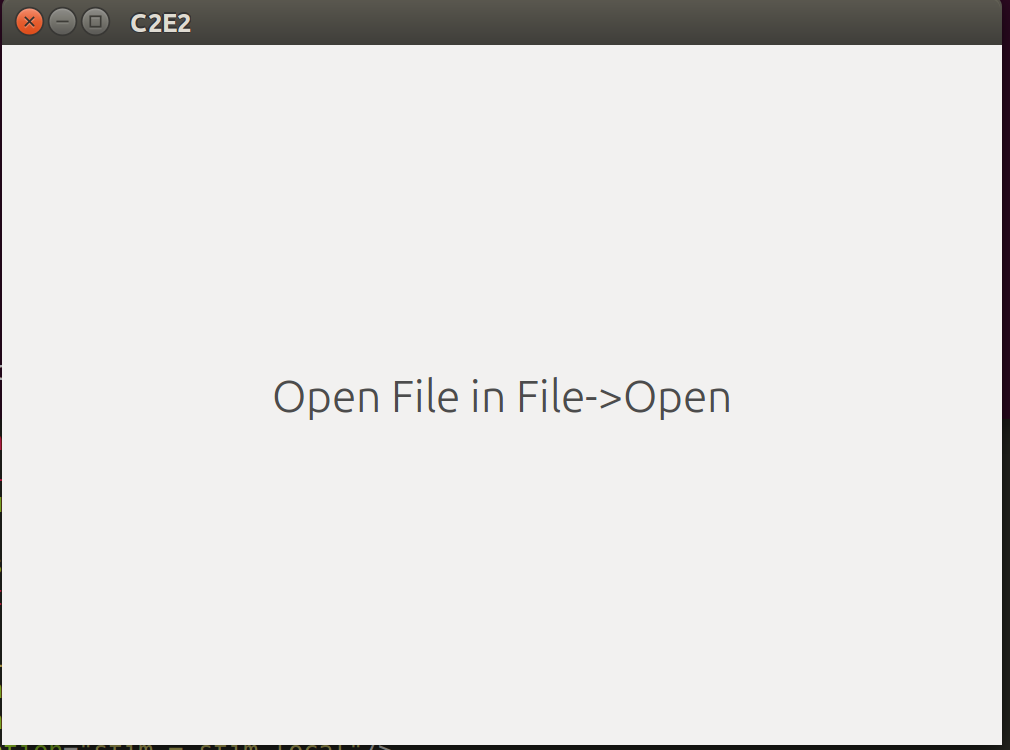
\includegraphics[scale=.24,keepaspectratio=true]{Manual_ver0_2_image/Frontend.png}}
 \caption{Frond end of C2E2 when launched} 
 \label{figure:frontend}
\end{marginfigure}

Upon opening the file , the C2E2 window should look like Figure~\ref{fig:parsetree}.  

\begin{figure}[h!]
\centerline{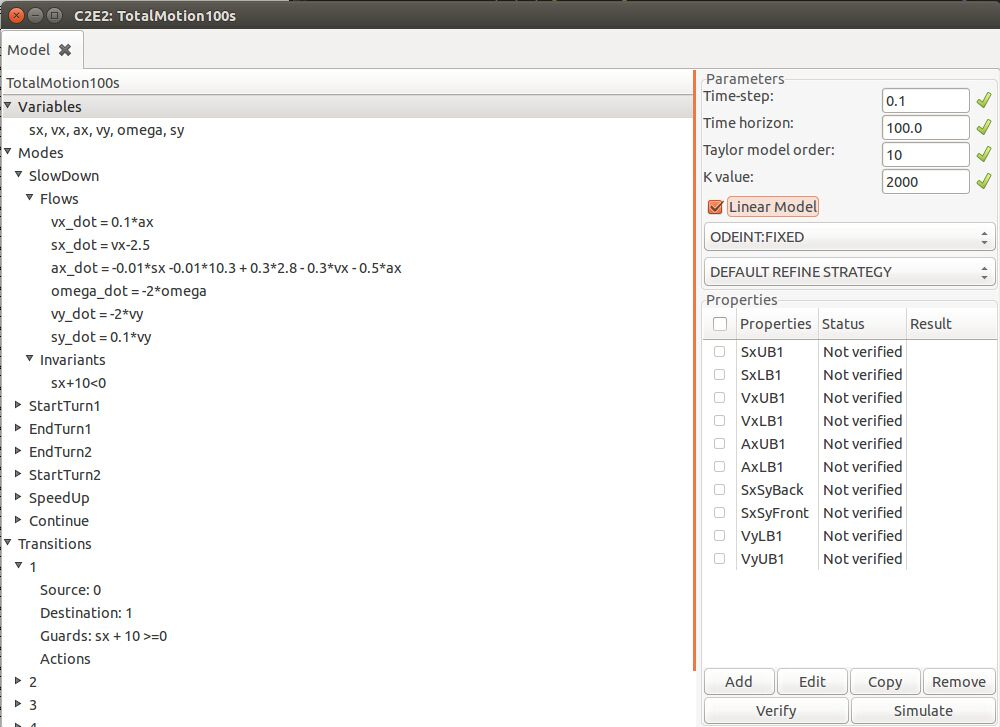
\includegraphics[scale=.22,keepaspectratio=true]{Manual_ver0_2_image/GUI.jpg}}
\caption{{\em Left:\/} Model parse tree. {\em Right:\/} Verification pane.} 
\label{fig:parsetree}
\end{figure}

The left hand side of this window shows the {\em parse tree \/}of the model
and the right hand side is the {\em verification pane\/}.
You can expand the tree to see the variables, dynamics, transitions and modes of the automaton by clicking on the arrows left.
In the near future, you will be able to edit the items in the parse tree. 
For now, this is a convenient representation of the model. 

If you want to use the default settings, please skip this section and go to Section~\ref{sec:properties} directly.

The coordinate transformation step $K$ for nonlinear models has been set to $2000$ by default at the top right corner of the verification pane. This value is important since the inappropriate $K$ value will influence the final result. The user can change the $K$ value to see different outputs.

~\newline
~\newline

\begin{itemize}
\item {Simulators}\\
Current version of C2E2 supports Odeint constant time step simulator, Odeint adaptive time step simulator and CAPD simulator. The default simulator is Odeint constant time step simulator, and it is been compiled when you opening the model. You can change the simulator by selecting different simulator from the simulator drop down menu as shown in Figure \ref{figure:simulator}. Note that the CAPD simulator may not work for several models due to the integration method used in the CAPD library. For example, the CAPD simulator for  \texttt{cardiacComposition.hyxml}, \texttt{Powertrain.hyxml}, \texttt{helicopter.hyxml} will fail simulating. 

\begin{marginfigure}
\centerline{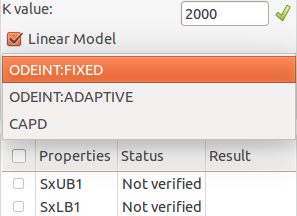
\includegraphics[scale=.24,keepaspectratio=true]{Manual_ver0_2_image/simulator.png}}
 \caption{Simulator drop down menu} 
 \label{figure:simulator}
\end{marginfigure}

\item {Refinement strategy}\\
When the initial set needs refinement, C2E2 provides different refinement strategies. The default refinement strategy will refine the dimensions within the unsafe set for four times, then iteratively refine the dimension with the largest uncertainty size. C2E2 also supports user defined strategy, which can be found at Section~\ref{sec:refinement_defined}. To select the strategy, please use the drop down menu on GUI as shown in Figure \ref{figure:refine}.


\begin{marginfigure}
\centerline{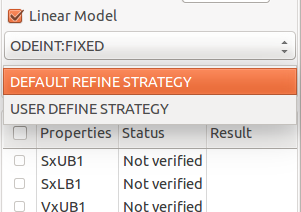
\includegraphics[scale=.24,keepaspectratio=true]{Manual_ver0_2_image/refine.png}}
 \caption{Refinement drop down menu} 
 \label{figure:refine}
\end{marginfigure}

\end{itemize}

\section{Properties}\label{sec:properties}

The right bottom corner of the main window is the property pane. 
This is where you can add, edit, copy properties and launch the verifier or simulator. 
Currently C2E2 verifies {\em bounded time linear invariant properties from linear bounded initial sets\/}.
Such properties are specified by the time bound ($T$), the initial set and the unsafe set. 
The {\em Time horizon\/} parameter listed at the top of the verification pane is the time bound.
%
Currently C2E2 requires both the initial and the unsafe sets to be described by a conjunction of linear inequalities involving the model variables.
The models in the \texttt{Examples} folder have already has a couple of sample properties.
Here we will walk you through the steps involved in creating a new property like in Figure~\ref{fig:property dialog}.

\begin{enumerate}
\item Click \texttt{Add} in the property pane. This launches the \texttt{Add Property} dialog box.
\item Enter a name for the property, say \texttt{VxLB1}, in the first textbox.
\item Enter a linear predicate on the variables to specify the {\em initial set\/} or the {\em starting states\/} in the second textbox. 
Currently, the syntax for specifying the initial set is as follows:\\
$\langle$ \texttt{mode-name} $\rangle$ : $\langle$ (\texttt{linear-inequality} \&\&)+ $\rangle$. \\
For example, for the above model: \\
\texttt{SlowDown}: sx>=-15.0 \&\& sx<=-14.95 
\&\& vx>=3.25 \&\& vx<=3.3 \&\& ax==0 \&\& vy==0
\&\& omega==0 \&\& sy==0  \\
is a valid expression for specifying the set of initial states. 
\item Enter the unsafe set in the last textbox.
Currently, the syntax for specifying the unsafe set is a \&\&-separated sequence of linear inequalities:\\
vx<=2.1 
\item Press \texttt{Add}.
\end{enumerate}
%
\begin{marginfigure}
\centerline{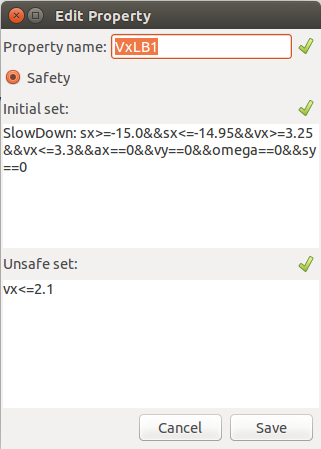
\includegraphics[width=\textwidth]{Manual_ver0_2_image/property_dialog.png}}
 \caption{Dialog box for adding properties checks the syntax of the initial and unsafe sets.}
 \label{fig:property dialog}
\end{marginfigure}
%
If all the expressions are syntactically acceptable then there will be little green checks
next to the textboxes and you will be able to save the property. Otherwise there will be a cross next to the textbox.
{\bf Both the unsafe set and the initial set should be described by a collection of linear inequalities and in addition the initial set should be bounded.\/}

Once the property is added the name of the property appears in the property pane. 
You may add several properties in the same way. 
You may also make copies of existing properties to save yourself some typing and edit them by clicking the \texttt{Edit} button.
The added properties can be saved with the model. See section~\ref{sec:loadsave}.

\section{Verifying}
\label{sec:verify}

Once you have created a model and added a property (see Section~\ref{sec:properties}) you can launch the verification engine by selecting the property and then clicking the \texttt{Verify} button.  


C2E2 is sound which means that you can trust the Safe/Unsafe answer proclaimed by it. 
In principle, C2E2 is also complete for robust properties~\citet{DMV13}. That is, if the 
model satisfies the property robustly\footnote{Robustness: the requirement that the actual reachable set of the model
does not skim the boundary of the unsafe set.}, and if the numerical precision supported by the 
algorithm is adequate then C2E2 should terminate with a Safe/Unsafe proclamation.
% 
In practice, the time it takes to verify is sensitive to the time horizon (T), the initial partition. 
You may want to first run the verification with small values of $T$ and initial set with small size.

The reachable set over-approximation computed by C2E2 is stored in the \texttt{/wd/ReachSet<Property name>}. You can also check the log file at \texttt{/wd/log} to check the progress of the verification. Once the verification is done, the result (Safe/Unsafe/Unknown) will show up at the Result column (as in Figure~\ref{fig:safe}). Note that if you see verification result as \texttt{Unknown}, it is because of the following reason:
\begin{enumerate}
\item The system is neither robustly safe nor robustly unsafe~\citet{DMV13}.
\item Reachable set computed bloats up and thus the number of refinements needed is too large. Please go back and check the model dynamic and properties, or simulate first to see whether the system trajectories bloats up.
\end{enumerate}


If you have multiple properties, then you may select one or more of them to be verified. Multiple properties are verified one at a time. When the verification is in progress clicking the \texttt{Abort} button aborts it.

\begin{marginfigure}
 \centerline{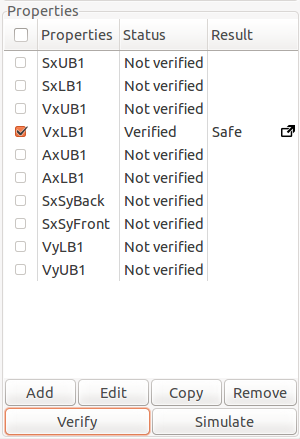
\includegraphics[scale=.25,keepaspectratio=true]{Manual_ver0_2_image/Verified.png}}
 \caption{One or more properties can be selected by checking the boxes to the left of the property name. The \texttt{Verify} button launches the verification engine to verify one property at a time.} 
 \label{fig:safe}
\end{marginfigure}


\subsection{Simulation}
C2E2 also allows users to generate pure simulation traces from initial sets. Once you have created a model and added a property (see Section~\ref{sec:properties}) you can launch the simulation engine by selecting the property and then clicking the \texttt{Simulate} button. C2E2 will select several states from initial set and generate simulation traces from those initial states. Note the Safe/Unsafe result shown in this case only stands for the safety of the simulation traces instead of all the reachable states from the initial set.

\subsection{User defined refinement strategy}\label{sec:refinement_defined}
C2E2 supports user defined refinement strategy (see Section ~\ref{sec:open}). You can select USER DEFINE STRATEGY from the drop down menu as shown in Figure \ref{figure:refine}. In this case, you need to write down your strategy in a file named \texttt{refineorder.txt} and store it in the \texttt{/wd} folder. The file should be look like Figure \ref{figure:refine_file}. In each line, you should write down the index of the variables, the order of which is the same as the variables that are shown in the front end GUI. That is, "2`` means the second variable shown in the Variables list in the front end. Indexes that are larger than the dimension of system will be ignored automatically. C2E2 will refine the initial set according to the order written in \texttt{refineorder.txt} iteratively. For example, if use the refinement strategy as in Figure~\ref{figure:refine_file}, the dimension corresponding to the second variable will be refined three times, then the dimension corresponding to the first variable will be refined once, then go back to the first line of \texttt{refineorder.txt} if the verification process has not terminated.

\begin{marginfigure}
 \centerline{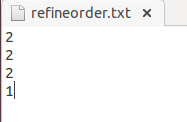
\includegraphics[scale=.25,keepaspectratio=true]{Manual_ver0_2_image/refine_order.png}}
 \caption{The user defined refine strategy file} 
  \label{figure:refine_file}
\end{marginfigure}


\subsection{Change Verified Properties}
Once a property is verified the status of the property will change to \texttt{Verified}, and the result \texttt{Safe/Unsafe/Unknown} will appear next to it. The verification result comes with a small box icon appears next to it to launch the plotter (see Section~\ref{sec:plots}). once the result has shown up, the property will be frozen temperately. At this point, if you change any of the parameters associated with the property, say the initial set or unsafe set, then the status of the property will change to \texttt{Verified*}. This (*) indicates that the property and parameters verified is outdated and you can launch the verifier again.


\section{Plotting}
\label{sec:plots}

Once the verification of a property is complete, a small box icon appears next to the result. Click this icon and this opens a new tab with the same name as the property. This is the plotting window for this property: it enables us to plot various projections of the reach set that has been computed in verifying the property. 
\begin{figure}[!htbp]
 \centerline{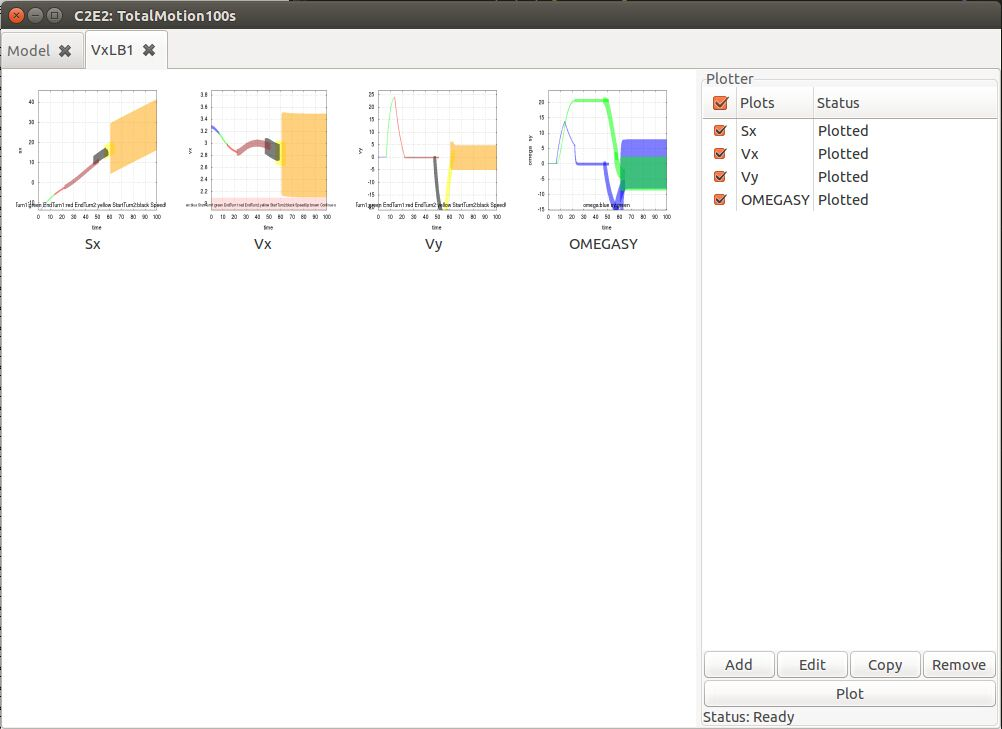
\includegraphics[scale=.25,keepaspectratio=true]{./Manual_ver0_2_image/Plot_display.jpg}}
 \caption{The plotting tab for property 1 without any plots.} 
\end{figure}
%
\newline
The plot window has two parts. 
The left pane shows all the plots icons and the right pane is used to create new plots. 
The steps for creating new plots (as in Figure~\ref{fig:plot_dialog}) is similar to that for creating properties:  
\begin{enumerate}
\item Click \texttt{Add} right bottom corner of the window. This launches the \texttt{Add Plots} dialog box.
\item Enter a name for the plot, say \texttt{Sx}, in the first textbox.
\item Select the x-axis and y-axis variable using the drop down menu, and add more y-axis variable if needed.
\item Click the \texttt{Save} button.
\end{enumerate}



\begin{marginfigure}
 \centerline{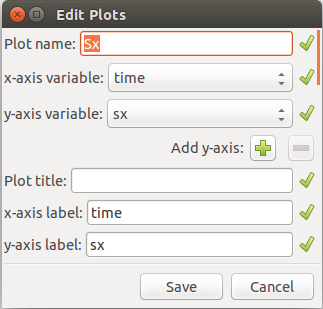
\includegraphics[scale=.24,keepaspectratio=true]{Manual_ver0_2_image/plot_dialog.png}}
 \caption{Add Plot dialog box.} 
 \label{fig:plot_dialog}
\end{marginfigure}


%
C2E2 can currently create two dimensional plots as Figure~\ref{fig:reachtube_plot}. As before, you can add more plots or edit/copy/remove/plots multiple plots. 
When you add/edit the plots, you will see a dialog box where you can select the variables would like to plot.
You can plot a state variable with respect to time (for example, x vs. t) or two state variables (x vx. y).
You can also plot multiple state variables with respect to time (x and y vs. t). 

Once you are satisfied with your plots, you can click the plot button generate the plots. 


As the program plots the reach sets, you will see icons appear on the left hand side of the window with a preview of what the plot looks like as well as the plot name below it. You can expand the plot by double clicking on these icons.

You can navigate the the first window and other opened plot windows by clicking on the tabs along the upper portion of the window. You can save the model as well as the properties you have created in an \texttt{.hyxml} file. 


Clicking on the \texttt{Plot} button will create 
the plots one by one and show the resulting icons.
Double click on an icon to expand a plot. The plot window allows you to pan and zoom over the reach tube and also generate \texttt{.png} figures of the plot in wd/plotresult folder.




\begin{marginfigure}
 \centerline{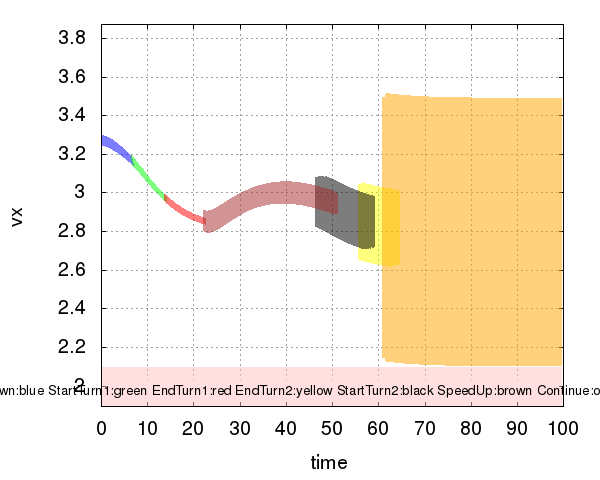
\includegraphics[scale=.24,keepaspectratio=true]{Manual_ver0_2_image/plot_open.png}}
 \caption{A plot of a reach tube of one variable with respect to time.} 
 \label{fig:reachtube_plot}
\end{marginfigure}

\subsection{Plots with multiple variables and modes}
\label{sec:multiplots}

If plotting multiple variables on the y-axis, the reach tube of each variable will be shown in different colors with labels. For example, in Figure~\ref{fig:xytime} the $x$-axis is time and the $y$-axis shows the reach tubes of two variables $\omega$ and $v_x$ which are shown in blue and green respectively. The axis for $v_x$ is labeled by green and that of $\omega$ is labeled by blue.

\begin{marginfigure}
 \centerline{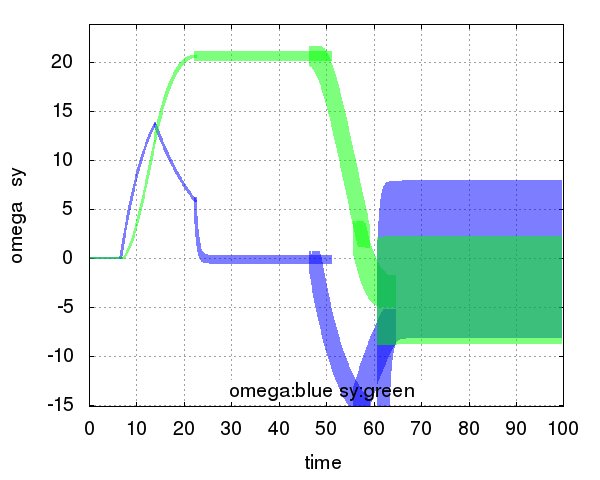
\includegraphics[scale=.24,keepaspectratio=true]{Manual_ver0_2_image/PLOT_RESULT_DOUBLE.png}}
 \caption{A plot of a reach tube of two variables with respect to time.} 
\label{fig:xytime}
\end{marginfigure}

\section{Loading and Saving}
\label{sec:loadsave}

Currently C2E2 provides very basic functionality for loading and saving models and properties. 
You can save a model and its properties from the file menu. 
The saved file is in the \texttt{.hyxml} format as shown below~\citet{SM:HSCC2011}.
Once saved, a model and the properties in the \texttt{.hyxml} file can be loaded from the file menu.

Changes made to the model in the C2E2 fronted are {\bf not\/} saved but only the edited properties are saved.
However, you can edit the \texttt{.hyxml} file using a text editor to change the model and the properties.
The reach sets computed during verification are stored in the working directory \texttt{/wd/} but currently they cannot be loaded.

\section{Format of HyXML}
\label{sec:hyxml}
Currently, C2E2 only accepts models of a certain form. The model can be defined in the HyXML file format - many examples of this can be found in the Examples/ directory. Multiple attributes must be defined for it to be a valid model. The attributes marked by * must be defined but are not used currently.
\begin{itemize}
\item automaton
	\begin{itemize}
	\item variable
    	\begin{itemize}
		\item name
		\item scope $\rightarrow$ LOCAL\_DATA, INPUT\_DATA, OUTPUT\_DATA
		\item type* $\rightarrow$ Real, Integer
        \end{itemize}
	\item mode (unique id's, consecutive order - 0 to n)
    	\begin{itemize}
        \item name
		\item initial $\rightarrow$ True, False
		\item dai $\rightarrow$ An equation of the form v\_out = algebraic formula if v is a local variable, else v = algebraic formula if v is an output variable
		\item invariant $\rightarrow$ Equation must be linear and use only local variables (Use \&lt; for <, etc)
		\end{itemize}
	\item transition
    	\begin{itemize}
		\item source, destination $\rightarrow$ IDs of modes
		\item id* $\rightarrow$ id of transition
		\item guard $\rightarrow$ Equation must be linear and use only local variables (Use \&lt; for <, etc)
		\item action (optional) $\rightarrow$ Can only use local variables and must be of the form v = linear formula
        \end{itemize}
    \end{itemize}
\item composition $\rightarrow$ automata should be a semicolon separated list of automata names you are composing
\item property
	\begin{itemize}
	\item unsafeSet $\rightarrow$ Conjunction of linear inequalities
	\item initialSet $\rightarrow$ <mode\_name>: Conjunction of linear inequalities
	\item name $\rightarrow$ verification/simulation data can be found at wd/ReachSet<name>
	\item type*
	\item parameters
    	\begin{itemize}
		\item taylororder $\rightarrow$ Taylor terms you want in the expansion
		\item timestep $\rightarrow$ Only used in ODE\_FIXED and CAPD
		\item timehorizon $\rightarrow$ Length of time you want to simulate for
		\item delta
        \end{itemize}
    \end{itemize}
\end{itemize}

\chapter{Using Command Line Version C2E2}

In this chapter, we give a quick introduction on running C2E2 using command line. We will use an example in the example folder.

In the c2e2 folder, type command ./runc2e2command to launch the command version C2E2 and you should able to see the model list (as in Figure~\ref{figure:terminalmain}). Command line version of C2E2 can only read models in the \texttt{Examples} folder. If you have customized models, please place it in the \texttt{Examples} folder as well. 
\newline

Once you load a file, C2E2 will start to compile simulator, and it will ask you to identify if it is a linear model or nonlinear model (see Figure~\ref{figure:terminallinear}). Type Y or N to answer, then the model will be successfully loaded.

Once the model is loaded, there will be various of commands you can use. Type \texttt{help} command to check the all the commands (see Figure~\ref{figure:terminalhelp}). These commands are similar to the functionality we have described in Section \ref{sec:open}. To check the properties that come with the \texttt{.hyxml} file, type \texttt{printprop} command. This command will expand all the built in properties as shown in Figure~\ref{figure:terminalprop}.By typing the \texttt{verify} command, you can verify all the properties in the property list. Results will be shown once the verification ends as in Figure~\ref{figure:terminalverify}.

When you are finishing with the command line version C2E2, you can type \texttt{quit} command to exit.

\begin{figure}
 \centerline{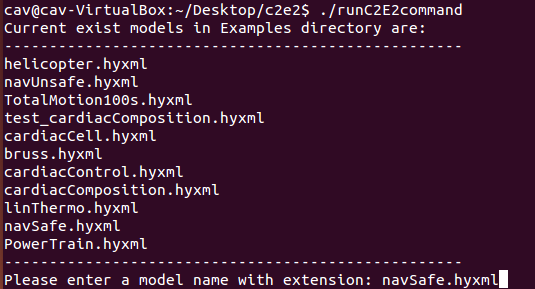
\includegraphics[scale=.25,keepaspectratio=true]{Manual_ver0_2_image/terminal_main.png}}
 \caption{Command line version C2E2 interface} 
  \label{figure:terminalmain}
\end{figure}

\begin{figure}
 \centerline{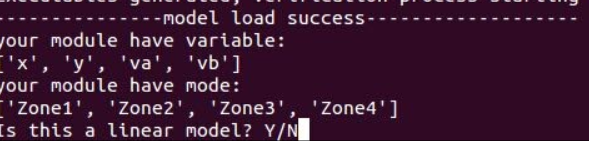
\includegraphics[scale=.25,keepaspectratio=true]{Manual_ver0_2_image/terminal_linear.png}}
 \caption{Type Y or N to tell C2E2 if the model is linear} 
  \label{figure:terminallinear}
\end{figure}

\begin{figure}
 \centerline{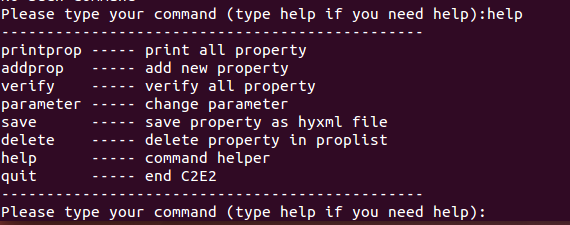
\includegraphics[scale=.25,keepaspectratio=true]{Manual_ver0_2_image/terminal_help.png}}
 \caption{All command options} 
  \label{figure:terminalhelp}
\end{figure}

\begin{figure}
 \centerline{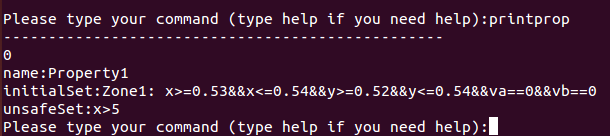
\includegraphics[scale=.25,keepaspectratio=true]{Manual_ver0_2_image/terminal_prop.png}}
 \caption{Expand properties come with the model \texttt{.hyxml} file} 
  \label{figure:terminalprop}
\end{figure}

\begin{figure}
 \centerline{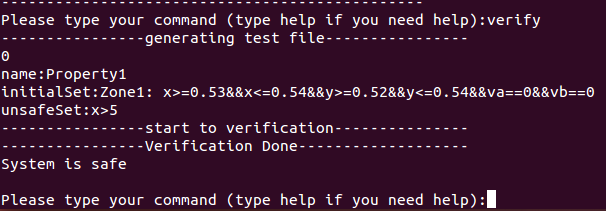
\includegraphics[scale=.25,keepaspectratio=true]{Manual_ver0_2_image/terminal_verify.png}}
 \caption{Verify the properties in the property list} 
  \label{figure:terminalverify}
\end{figure}





\appendix
\chapter{Required Libraries}
\label{app:packs}
The following is a complete list of packages needed for installing C2E2. 
\begin{enumerate}
 \item GNU Linear Programming Kit along with Python bindings, GLPK and PyGLPK (http://www.gnu.org/software/glpk/) (http://tfinley.net/software/pyglpk/)
 \item GNU parser generator, Bison (http://www.gnu.org/software/bison/)
 \item The Fast Lexical Analyzer, Flex (http://flex.sourceforge.net/) 
 \item Python (http://www.python.org/)
 \item Python parsing libraries, Python-PLY (http://code.google.com/p/ply/)
 \item GTK libraries for Python (http://www.pygtk.org/)
 \item Plotting libraries for Python, Matplotlib (http://matplotlib.org/)
 \item Packing configurations library  (http://www.freedesktop.org/wiki/Software/pkg-config/)
 \item GNU Autoconf (http://www.gnu.org/software/autoconf/)
 \item Python xml library, lxml (http://lxml.de/installation.html)
 \item Parma Polyhedron Library (http://bugseng.com/products/ppl/)
 \item Python Sympy library (http://www.sympy.org/en/index.html)
 \item Boost libraries (http://www.boost.org)
\end{enumerate}

If you get any errors while installing PyGLPK, please visit the following website:\\ \url{http://tfinley.net/software/pyglpk/building.html} and install it manually.

\backmatter

%----------------------------------------------------------------------------------------
%	BIBLIOGRAPHY
%----------------------------------------------------------------------------------------

\bibliography{sayan1} % Use the bibliography.bib file for the bibliography
\bibliographystyle{plainnat} % Use the plainnat style of referencing

%----------------------------------------------------------------------------------------

\printindex % Print the index at the very end of the document

\end{document}